% Options for packages loaded elsewhere
\PassOptionsToPackage{unicode}{hyperref}
\PassOptionsToPackage{hyphens}{url}
%
\documentclass[
]{article}
\usepackage{amsmath,amssymb}
\usepackage{iftex}
\ifPDFTeX
  \usepackage[T1]{fontenc}
  \usepackage[utf8]{inputenc}
  \usepackage{textcomp} % provide euro and other symbols
\else % if luatex or xetex
  \usepackage{unicode-math} % this also loads fontspec
  \defaultfontfeatures{Scale=MatchLowercase}
  \defaultfontfeatures[\rmfamily]{Ligatures=TeX,Scale=1}
\fi
\usepackage{lmodern}
\ifPDFTeX\else
  % xetex/luatex font selection
\fi
% Use upquote if available, for straight quotes in verbatim environments
\IfFileExists{upquote.sty}{\usepackage{upquote}}{}
\IfFileExists{microtype.sty}{% use microtype if available
  \usepackage[]{microtype}
  \UseMicrotypeSet[protrusion]{basicmath} % disable protrusion for tt fonts
}{}
\makeatletter
\@ifundefined{KOMAClassName}{% if non-KOMA class
  \IfFileExists{parskip.sty}{%
    \usepackage{parskip}
  }{% else
    \setlength{\parindent}{0pt}
    \setlength{\parskip}{6pt plus 2pt minus 1pt}}
}{% if KOMA class
  \KOMAoptions{parskip=half}}
\makeatother
\usepackage{xcolor}
\usepackage[margin=1in]{geometry}
\usepackage{graphicx}
\makeatletter
\newsavebox\pandoc@box
\newcommand*\pandocbounded[1]{% scales image to fit in text height/width
  \sbox\pandoc@box{#1}%
  \Gscale@div\@tempa{\textheight}{\dimexpr\ht\pandoc@box+\dp\pandoc@box\relax}%
  \Gscale@div\@tempb{\linewidth}{\wd\pandoc@box}%
  \ifdim\@tempb\p@<\@tempa\p@\let\@tempa\@tempb\fi% select the smaller of both
  \ifdim\@tempa\p@<\p@\scalebox{\@tempa}{\usebox\pandoc@box}%
  \else\usebox{\pandoc@box}%
  \fi%
}
% Set default figure placement to htbp
\def\fps@figure{htbp}
\makeatother
\setlength{\emergencystretch}{3em} % prevent overfull lines
\providecommand{\tightlist}{%
  \setlength{\itemsep}{0pt}\setlength{\parskip}{0pt}}
\setcounter{secnumdepth}{-\maxdimen} % remove section numbering
% definitions for citeproc citations
\NewDocumentCommand\citeproctext{}{}
\NewDocumentCommand\citeproc{mm}{%
  \begingroup\def\citeproctext{#2}\cite{#1}\endgroup}
\makeatletter
 % allow citations to break across lines
 \let\@cite@ofmt\@firstofone
 % avoid brackets around text for \cite:
 \def\@biblabel#1{}
 \def\@cite#1#2{{#1\if@tempswa , #2\fi}}
\makeatother
\newlength{\cslhangindent}
\setlength{\cslhangindent}{1.5em}
\newlength{\csllabelwidth}
\setlength{\csllabelwidth}{3em}
\newenvironment{CSLReferences}[2] % #1 hanging-indent, #2 entry-spacing
 {\begin{list}{}{%
  \setlength{\itemindent}{0pt}
  \setlength{\leftmargin}{0pt}
  \setlength{\parsep}{0pt}
  % turn on hanging indent if param 1 is 1
  \ifodd #1
   \setlength{\leftmargin}{\cslhangindent}
   \setlength{\itemindent}{-1\cslhangindent}
  \fi
  % set entry spacing
  \setlength{\itemsep}{#2\baselineskip}}}
 {\end{list}}
\usepackage{calc}
\newcommand{\CSLBlock}[1]{\hfill\break\parbox[t]{\linewidth}{\strut\ignorespaces#1\strut}}
\newcommand{\CSLLeftMargin}[1]{\parbox[t]{\csllabelwidth}{\strut#1\strut}}
\newcommand{\CSLRightInline}[1]{\parbox[t]{\linewidth - \csllabelwidth}{\strut#1\strut}}
\newcommand{\CSLIndent}[1]{\hspace{\cslhangindent}#1}
\usepackage{setspace}
\usepackage{bookmark}
\IfFileExists{xurl.sty}{\usepackage{xurl}}{} % add URL line breaks if available
\urlstyle{same}
\hypersetup{
  pdftitle={Normalizations are not what you think; Explicit Scale Simulation in ALDEx2},
  hidelinks,
  pdfcreator={LaTeX via pandoc}}

\title{Normalizations are not what you think; Explicit Scale Simulation
in ALDEx2}
\author{true \and true \and true}
\date{}

\begin{document}
\maketitle
\begin{abstract}
In high-throughput sequencing (HTS) studies, sample-to-sample variation
in sequencing depth is driven by technical factors, and not by variation
in the scale (e.g., total size, microbial load, or total gene
expression) of the underlying biological systems. Typically a
statistical normalization is used to remove unwanted technical variation
in the data or the parameters of the model to enable analyses that are
sensitive to scale; e.g., differential abundance and differential
expression analyses. Recently we showed that all normalizations make
implicit assumptions about the unmeasured system scale and that errors
in these assumptions can lead to dramatic increases in false positive
and false negative rates. Here we describe updates to the ALDEx2 R
package that mitigate these problems by directly modeling uncertainty in
the unmeasured system scale through the use of a \textit{scale model}.
Scale models generalize the idea of normalizations and can be thought of
as explicitly modeling the error in normalization by examining a
distribution over all possible normalizations. Beyond enhancing the
robustness of HTS analyses, the use of scale models within ALDEx2
enhances the transparency and reproducibility of analyses by making
implicit normalizing assumptions an explicit part of the model building
process.
\end{abstract}

\section{Introduction}\label{introduction}

High-throughput sequencing (HTS) is a ubiquitous tool used to explore
many biological phenomenon such as gene expression (single-cell
sequencing, RNA-sequencing, meta-transcriptomics), microbial community
composition (16S rRNA gene sequencing, shotgun metagenomics) and
differential enzyme activity (selex, CRISPR killing). HTS proceeds by
taking a sample from the environment, making a library, multiplexing
(merging) multiple libraries together, and then applying a sample of the
multiplexed library to the flow cell. Each of these steps is a
compositional sampling step as only a fixed-size subsample of nucleic
acid is carried over to subsequent steps. Thus, with each sampling step
the connection between the size of the sampled DNA pool and the scale
(e.g., size, microbial load, or total gene expression) of the measured
biological system is degraded or lost. Increasingly, researchers are
turning to modified experimental protocols (e.g., DNA spike-ins or cell
counting) in an attempt to recover the lost biological variation in
scale; see for example (1, 2). However, these protocols often do not
recover meaningful biological variation but instead recover scale
variation at the intermediate step in the sample preparation protocol
where the DNA spike-in was added. In short, the disconnect between
sample-to-sample variation in sequencing depth and biological variation
in scale remains an outstanding challenge.

The analysis of HTS data suffers from several known problems that can be
traced, in whole or in part, to misspecification of scale. The first
issue is poor control of the false discovery rate (FDR)
{[}(3);(4);Nearing:\href{mailto:2022aa;@Li}{\nolinkurl{2022aa;@Li}}:2022aa{]},
exhibited as dataset-dependent FDR control. The FDR problem is connected
to the double-filtering approach that is often used, but which is known
not to have appropriate FDR control (5, 6). The second issue is poor
performance when analyzing asymmetric data; data that arises because of
a bias in the direction of change. This type of data frequently arises
in in-vitro selection experiments (SELEX), transcriptome analysis, and
microbiome analysis (7). The third issue is that these problems become
more pronounced as more samples are collected; that is, more information
results in a worsening of the accuracy of the analysis (9). The final
problem is that these data are relative data, i.e.~compositional (10,
11), and substantial effort has been put into removing this constraint.

The first three problems were recently shown by Nixon and Silverman (8)
to be a result of a mismatch between the underlying size or scale of the
system and the assumptions of the normalizations used for the analysis
of HTS. Biological variation in scale often represents an important
unmeasured confounder in HTS analyses (12). For example, cells
transformed by the cMyc oncogene have about 3 times the amount of mRNA
and about twice the rRNA content than non-transformed cells (13), and
this dramatically skews transcriptome analysis (14). In addition,
wild-type and mutant strains of cell lines, yeast or bacteria have
different growth rates and RNA contents under different conditions,
which affect our ability to identify truly differentially abundant genes
(15--17). As another example, the total bacterial load of the vaginal
microbiome differs by 1-2 orders of magnitude in absolute abundance
between the healthy and bacterial vaginosis states (18), and the
composition between these states is dramatically different (19, 20).
Thus, a full description of any of these systems includes both relative
change (composition) and absolute abundance (scale). Current methods
access only the compositional information yet make implicit assumptions
about the scale.

Recently, Nixon et al. (8) showed that the challenge of non-biological
variation in sequencing depth be viewed as a problem of
partially-identified models. They showed that \emph{all} normalizations
make some assumption about scale. These implicit assumptions are often
difficult to interpret, and different normalizations provide different
outputs when applied to the same dataset (3, 21--24). Intuitively,
normalizations in widespread use assume that either all samples have the
same scale, e.g.~proportions, rarefaction (25), RPKM (26, 27), etc; or
that a subset of features in one sample can be chosen as a reference to
which the others are scaled e.g.~the TMM (28), or LVHA (7) or the
additive log-ratio (29); or that different sub-parts of each sample
maintain a constant scale across samples e.g.~the RLE (30); or that the
geometric mean of the parts is appropriate e.g the CLR and its
derivatives.

The original ALDEx2 (31) model unwittingly made a strict assumption
about scale through the CLR normalization (8). While this assumption
could be useful in many cases it could never be exactly true, and others
have shown that it is not always the best option (32). Nixon et al. (8)
showed that better scale assumptions resulted in more reproducible data
analysis including better control of both false positive and false
negative results. In essence ALDEx2 has been modified to explicitly
model the scale over a range of reasonable normalization parameters.
Here, we briefly introduce these modifications and then show how scale
uncertainty can greatly improve modeling in transcriptome and
meta-transcriptome datasets to provide more robust and reproducible
results.

\section{Implementation}\label{implementation}

To be concrete, we let \(\mathbf{Y}\) denote the \emph{measured}
\(D \times N\) matrix of sequence counts with elements
\(\mathbf{Y}_{dn}\) indicating the number of measured DNA molecules
mapping to feature \(d\) (e.g., a taxon or gene) in sample \(n\).
Likewise, we can denote \(\mathbf{W}\) as the \emph{true} amount of
class \(d\) in the biological system from which sample \(n\) was
obtained. We can think of \(\mathbf{W}\) as consisting of two parts, the
scale \(\mathbf{W}^{\perp}\) (e.g., totals) and the composition
\(\mathbf{W}^{\parallel}\) (i.e., proportions). That is,
\(\mathbf{W}^{\perp}\) is a \(N\)-vector with elements
\(\mathbf{W}^{\perp}_{n}=\sum_{d}\mathbf{W}_{dn}\) while
\(\mathbf{W}^{\parallel}\) is a \(D \times N\) matrix with elements
\(\mathbf{W}^{\parallel}_{dn}=\mathbf{W}_{dn}/\mathbf{W}^{\perp}_{n}\).
Note that with these definitions \(\mathbf{W}\) can be written as the
element-wise combination of scale and composition:
\(\mathbf{W}_{dn}=\mathbf{W}^{\parallel}_{dn}\mathbf{W}^{\perp}_{n}\).

All the normalizations in current use are data transformations that can
be stated as ratios of the form
\(\hat{{\mathbf{W}}}_{dn}=\mathbf{Y}_{dn}/f(\mathbf{Y})\), where the
denominator is determined by some function of the observation. We use
the \(\hat{{\mathbf{W}}}\) notation to indicate that the normalization
is attempting to provide an estimate of the true value. The technical
variation in sequencing depth
(\(\mathbf{Y}^{\perp}_{n}=\sum_{d}\mathbf{Y}_{dn}\)) implies that
observed data \(\mathbf{Y}\) provides us with information about the
system composition \(\mathbf{W}^{\parallel}\) but little to no
information in the system scale \(\mathbf{W}^{\perp}\) (Lovell et
al.~2011).

\subsection{Adding Scale Uncertainty in
ALDEx2}\label{adding-scale-uncertainty-in-aldex2}

The ALDEx2 R package (31, 33) is a general purpose toolbox for Bayesian
modeling of HTS data. For brevity, we discuss ALDEx2 in its simplest
form as a tool for estimating the magnitude and statistical significance
of Log-Fold-Changes (LFC) (e.g., differential abundance or differential
expression analysis), but note that it can be used to fit more complex
linear models. At a high-level, ALDEx2 involves three steps: 1) a
Bayesian model is used to estimate \(\mathbf{\hat{W}}^{\parallel}\)
given observations \(\mathbf{Y}\); 2) a normalization is used to
estimate \(\mathbf{\hat{W}}\) given the estimate
\(\mathbf{\hat{W}}^{\parallel}\); 3) the \(\mathbf{\hat{W}}\) estimates
are used to estimate LFC as part of differential abundance (or
expression) analyses. For more details on ALDEx2 see (8, 31).

By default, ALDEx2 uses the CLR normalization which can be written as
\(\log \mathbf{\hat{W}}_{dn}=\log (\mathbf{\hat{W}}^{\parallel}_{dn}/G_{n})\)
where \(G_{n}\) denotes the geometric mean of the vector
\((\hat{W}^{\parallel}_{1n}, \dots, \hat{W}^{\parallel}_{Dn})\). The CLR
normalization equates to an implicit assumption that
\(\mathbf{\hat{W}}^{\perp}_{n}=1/G_{n}\)(8) and even slight errors in
this assumption introduces bias into the LFC estimate that is not
accounted for when estimating uncertainty (e.g., confidence intervals or
credible sets). In fact, Nixon et al. (8) showed that the only way in
which the ALDEx2 model, or any normalization-based model, could ever be
calibrated (e.g., control Type-I Error rates) was if this assumption was
exactly true. In support of this assertion it is known that false
discovery rates vary widely by analysis, dataset, and normalization
method (34, 35). To fix this, Nixon et al. (8) showed that models should
incorporate potential error in the assumptions implied by
normalizations.

Nixon et al.~(2023) generalized the concept of normalizations by
introducing the concept of a \textit{scale model} to account for
potential error. Scale models can be incorporated into ALDEx2, turning
the ALDEx2 model into a specialized type of statistical model which they
called a \textit{Scale Simulation Random   Variable} (SSRV). They did
this by including a model for \(\mathbf{\hat{W}}^{\perp}_{n}\). Since
the CLR normalization makes the assumption
\(\mathbf{\hat{W}}^{\perp}_{n}=1/G_{n}\), the CLR normalization can be
generalized by considering probability models for the scale
\(\mathbf{\hat{W}}^{\perp}_{n}\) that have mean \(1/G_{n}\). For
example, the following scale model generalizes the CLR:

\[\log \mathbf{\hat{W}}^{\perp}_{n} = -\log G_{n} + \Lambda x_{n} \qquad \Lambda \sim N(0, \gamma^{2})\]

where \(\gamma\) is a tunable parameter drawn from a Gaussian
distribution that controls the degree of uncertainty in the CLR
assumption and \(x_{n}\) denotes a binary condition indicator (e.g.,
\(x_{n}=1\) denotes case and \(x_{n}=0\) denotes control). We have made
those modifications a permanent fixture of ALDEx2 which now represents
the first software package designed for SSRV-based inference.

\section{Results}\label{results}

\subsection{Adding scale uncertainty replaces the need for dual
significance
cutoffs.}\label{adding-scale-uncertainty-replaces-the-need-for-dual-significance-cutoffs.}

It is standard practice in many fields of HTS, but especially
transcriptomics, to use the dual cutoff approach graphically exemplified
by volcano plots (36, 37) because not all statistically significant
differences are biologically relevant. Paraphrasing this we can say that
in in some types of datasets more samples leads to a majority of
features being statistically significant. A detailed reasoning for this
using modelled data is explained in two reports by Nixon et al. (8, 9),
which shows that scaled models completely address this analytic issue.

We use the data of Gierliński et al. (38) who conducted a highly
replicated yeast transcriptome experiment comparing a wild-type strain
with a snf2 gene knockout, \(\Delta\)snf2. This dataset has been used to
argue that a dual cutoff approach is appropriate to limit the number of
significant parts and for purposes of reproducibility (37). However, in
this benchmarking study, the number of significantly different
transcripts varied between 65\% to \textgreater80\% of all transcripts
depending on the tool; in essence the desired behavior was that almost
all transcripts were significantly different. The guidance on
reproducibility runs counter to standard statistical practice where
power is intrinsically linked to sample size and very large sample sizes
are indeed desired (39). Furthermore, the dual-cutoff approach is known
not to provide appropriate FDR control (5, 6). Schurch et al. (37)
further suggested that different tools might be better in some
conditions or datasets than others because each tool has different
intrinsic statistical power and Type 1 and Type 2 errors. Through the
lens of scale uncertainty, the behaviour of the tools in this study show
unacknowledged bias; false confidence in the precision of the estimate
as sample size increases because o mis-specification in the scale of the
data. This certainty is driven by the assumptions of the tool not the
actual experiment being investigated (9).

Using either DESeq2 or ALDEx2, a majority of transcripts are
statistically significantly different between groups with a
Benjamini-Hochberg (40) false discovery rate (FDR) of 0.05; i.e.~4636
(79\%, DESeq2) or 4172 (71\%, ALDEx2) of the 5891 transcripts. Such
large numbers of significant transcripts seems biologically unrealistic
and furthermore breaks the necessary assumption made by the
normalization methods that the majority of the features must be
invariant. That 118 transcripts are identified by ALDEx2 and not DESeq2,
while DESeq2 identifies 582 transcripts that ALDEx2 does not, suggests
that the choice of normalization plays a role in which results are
returned as significant and that some if not the majority are driven by
technical differences in the analysis (22, 23, 37, 41, 42).

\begin{figure}
\centering
\pandocbounded{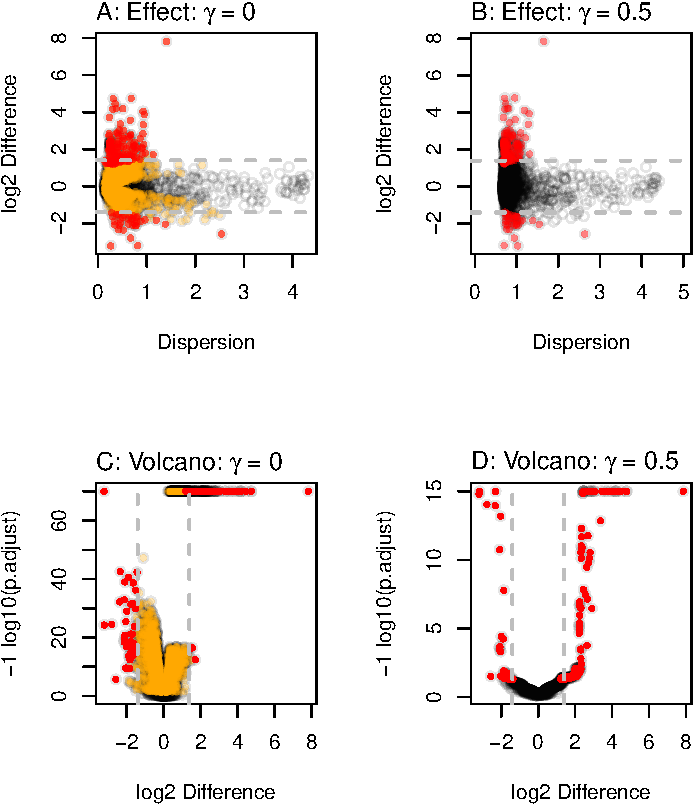
\includegraphics[keepaspectratio]{go3_files/figure-latex/plot1-1.pdf}}
\caption{Effect and volcano plots for unscaled and scaled transcriptome
analysis. ALDEx2 was used to conduct a differential abundance (DA)
analysis on the yeast transcriptome dataset. The results were plotted to
show the relationship between difference and dispersion using effect
plots ) or difference and the Benjamini-Hochberg corrected p-values
(volcano plot). Panels A,C are for the unscaled analysis, and Panels B,D
are for the scaled analysis. Each point represents the values for one
transcript, with the color indicating if that transcript was significant
in the scaled analysis and unscaled analysis (red) or in the unscaled
analysis only (orange). Points in grey are not statistically
signficantly different with any analysis. The horizontal dashed lines
represent a log2(difference) of \(\pm 1.4\).}
\end{figure}

The effect plots (43) in Figure 1A (ALDEx2) and Supplementary Figure 1
(DESeq2) shows that the majority of significant transcripts (red,
orange) have negligible differences between groups and very low
dispersion and we suggest that this is driven by the experimental design
(37). Scale uncertainty can be incorporated using the \texttt{gamma}
parameter that controls the amount uncertainty added to the CLR mean
assumption when we call either \texttt{aldex()}, or
\texttt{aldex.clr()}. Figure 1B shows that setting \(\gamma=0.5\)
results in far fewer transcripts being significant (205) and we observe
that the minimum dispersion increases from 0.12 (unscaled) to 0.67
(scaled). The Volcano plots in Figure 1 C and D show a similar story.
Here we can see that adding scale increases the minimum FDR value and
increases the concordance between the FDR value and the difference
between groups (compare panels C and D).

\begin{figure}
\centering
\pandocbounded{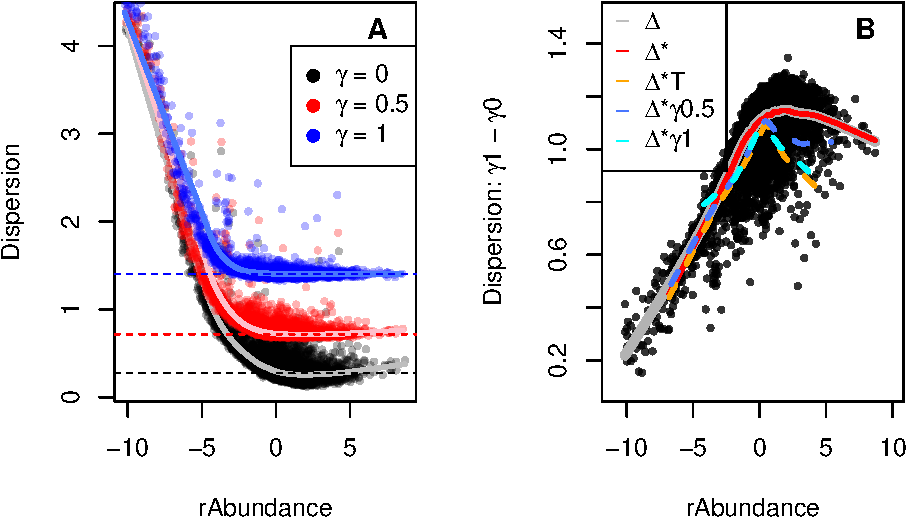
\includegraphics[keepaspectratio]{go3_files/figure-latex/disp-1.pdf}}
\caption{Adding scale uncertainty changes the dispersion distribution.
Panel A shows a plot of the expected value for relative abundance vs the
expected value for the pooled dispersion as output by
\texttt{aldex.effect}. The dashed horizontal lines show the median value
for the features with a rAbundance between -0.5 and 0.5, and the light
colored lines are lowess lines of fit through the center of mass of the
data. Panel B plots the dispersion difference between \(\gamma = 1\) and
\(\gamma = 0\); note the non-linear relationship that highlights the
rotation that is evident in Panel A. The colored lines indicate the
lowess line of fit through the centre of mass of the plot for the
various populations of points. The grey line is the total population and
shows the difference \(\Delta\), the red line is the population of
significant transcripts (*) with no scale, the orange line is the
population of significant transcripts with a difference threshold (T) of
about \(\pm 2^{1.4}\)-fold change, the blue line is the population of
significant transcripts with \(\gamma = 0.5\), and the cyan line is the
significant population with \(\gamma = 1\). \(\Delta\): Difference, *:
significant, T: thresholded.}
\end{figure}

As shown by the effect plot in Figure 1 the root cause of the many
statistically significant positive transcripts is the very large number
of transcripts with negligible variance. This phenomenon is not unique
to ALDEx2 as Supplementary Figure 1 shows that the same phenomenon
occurs in DESeq2 (and presumably other methods although the relevant
parameters are not exposed). This issue is not unique to this dataset
and it is common practice to use a dual-cutoff by choosing transcripts
based on a thresholds for both corrected p-values and fold-changes (37)
(here set at \(\pm 2^{1.4}\) for the latter), although considerable
variation in cutoff values is observed. These limits are shown by the
dashed grey lines. Here, applying a dual-cutoff using a heuristic of at
least a \(2^{1.4}\) fold change reduces the number of significant
outputs to 193 for DESeq2 and to 186 for ALDEx2, and is in-line with
that observed with that found by ALDEx2 with \(\gamma = 0.5\) which
identifies 205. Indeed, Supplementary Figure 2, shows that even adding a
very small amount of scale \(\gamma = 0.1\) reduces the number of
significant transcripts by more than half and the
\texttt{aldex.scaleSim()} function can be used to identify those
transcripts that are significant only because of an absence of scale.
These results begs the question: why bother with significance tests at
all if all transcripts with \(> 1.4\)-fold expression change are
statistically significant?

The effect on dispersion with increasing amounts of scale are shown in
Figure 2A, where we can see that the dispersion increases as scale is
added. Note that the dispersion in the unscaled data in Figure 2A
reaches a minimum near the mid-point of the distribution, and also does
so when the analysis is conducted with DESeq2 (Supplementary Figure 3).
This shows more clearly that dispersion of many transcripts is almost
negligible in the absence of scale and makes the counter-intuitive
suggestion that the variance in expression of the majority of genes with
moderate expression is more predictable than highly-expressed genes or
of housekeeping genes (44). This is at odds with the known biology of
cells where single cell counting of highly-expressed transcripts shows
that they have little intrinsic variation (45).

Adding scale by setting \(\gamma=0.5\) , or \(\gamma = 1.0\), increases
the minimum dispersion as shown in Figure 2A by the red and blue data
points, and by the colored lines of fit through the centre of mass of
the data. Less obvious is that the scaled dispersion estimates are
rotated. Figure 2B shows a plot of the difference between the
\(\gamma= 0\) and \(\gamma= 1\) data to show this more clearly and here
we can see that the scale is preferentially increasing the dispersion of
the mid-expressed transcripts that formerly had negligible dispersion;
examine the grey line of best fit (overlaid by the red line) for the
trend. Panel B also shows the trend of the expression-dispersion
relationship for transcripts that are classed as statistically
significant. The red line shows the trendline with no added scale, and
this trendline exactly overlays with the grey trendline of the bulk of
transcripts. The orange trendline indicates those transcripts that are
both statistically significant and that have a thresholded expression
level of \(\pm 1.4\), and the dark blue and cyan lines show the
statistically significant trendline for \(\gamma=0.5\) , or \(1.0\).
Note that this has the effect of changing the distribution of parts
identified as significant and that the substantially fewer significantly
different genes are in the very high abundance but low dispersion
category.

\subsection{Housekeeping genes can be used to guide scale model
choices.}\label{housekeeping-genes-can-be-used-to-guide-scale-model-choices.}

Dos Santos et al. (46) used a vaginal metatranscriptome dataset to
compare the gene expression in bacteria collected from healthy (H) and
bacterial vaginosis (BV) affected women. In this environment, both the
relative abundance of species between groups and the gene expression
level within a species is different (47). Additionally, prior research
suggests that the total number of bacteria is about 10 times more in the
BV than in the H condition (18). Thus, this is an extremely challenging
environment in which to determine differential abundance as there are
both compositional and scale changes between conditions. The usual
method to analyze vaginal metratranscriptome data is on a taxon-by-taxon
basis (47--49) because the scale confounding can be ignored. Attempts at
system-wide analysis show that many housekeeping functions are returned
as differentially abundant between groups; a result likely due to a
disconnect between the scale assumptions of the normalization used (7).

In this example, we show how to specify a user-defined, or
\emph{informed}, scale model explicitly that can account for some of
these modeling difficulties. An informed scale model can control for
both the mean difference of scale between groups (e.g., directly
incorporate information on the differences in total number of bacteria
between the BV and H conditions) as well as the uncertainty assumed in
that difference. To specify a user-defined scale model, we can pass a
matrix of scale values instead of a single estimate of gamma to
\texttt{aldex.clr()}. This matrix should have the same number of rows as
the of Monte-Carlo Dirichlet samples, and the same number of columns as
the number of samples. While this matrix can be computed from scratch by
the analyst, there is an \texttt{aldex.makeScaleModel()} function that
can be used to simplify this step in most cases. This encodes the scale
model as \(\Lambda \sim N(log2 \mu_n, \gamma^{2})\), where \(\mu_n\)
represents the actual scale value for each sample. This can be a
measured value (cell count, nucleic acid input, etc), or an imputed
value. Nixon et al. (9) showed that only the ratio between the scale
values for each sample was important; see Supplementary Figures 4 and 5
for a demonstration of this point.

Figure 3A shows an effect plot of the data where reads are grouped by
function, corresponding to grouping homologous sequences regardless of
the organism of origin. Each point represents one of 3728 KEGG functions
(50). There are many more functions represented in the BV group (bottom)
than in the healthy group (top). This is because the
\textit{Lactobacilli} that dominate a healthy vaginal microbiome have
reduced genome content relative to the anaerobic organisms that dominate
in BV, because there is a greater diversity of organisms in BV than in H
samples, and because the BV condition has at least an order of magnitude
more bacteria than does the H condition.

There are 101 functions with low dispersion that appear to be share by
both groups (boxed area in Figure 3A, and colored in cyan). Inspection
shows that these largely correspond to core metabolic functions such as
transcription, translation, ribosomal proteins, glycolysis, replication,
chaperones, etc (Supplementary file housekeeping.txt). The transcripts
of many of these are commonly used as invariant reference sequences (44)
and so would not be expected to contribute to differences in ecosystem
behaviour and should be centred on 0 difference. These should not be
scored as among the most differentially abundant. The major group of
these housekeeping functions is located off the line of no difference
(being approximately located at +1.5). While changes in the abundance of
housekeeping functions is a useful proxy for relative abundance of
species in the environment, they tell us nothing about the functional
capacity of the two groups as these are common to every organism. Of
more interest is determining the functions that are different between
groups because these are unique or over-expressed in one group relative
to the other.

\begin{figure}
\centering
\pandocbounded{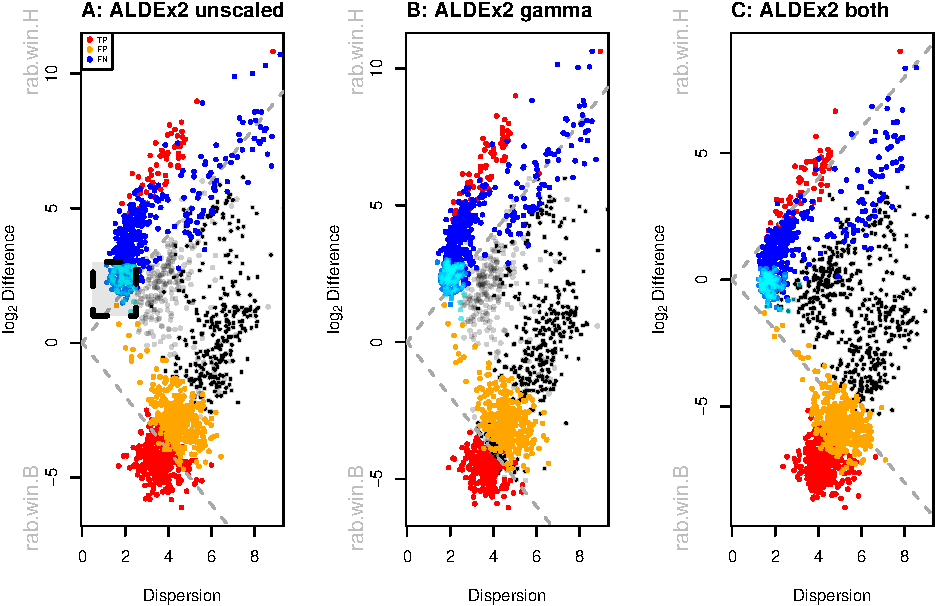
\includegraphics[keepaspectratio]{go3_files/figure-latex/meta-1.pdf}}
\caption{Analysis of vaginal transcriptome data aggregated at the Kegg
Orthology (KO) functional level. Panel A shows an effect plot for the
default analysis where the functions that are elevated in the healthy
individuals have positive values and functions that are elevated in BV
have negative values. Highlighed in the box are KOs that are almost
exlusively housekeeping functions and are colored cyan. These
housekeeping functions should be located on the midline of no
difference. Panel B shows the same data scaled with \(\gamma = 0.5\),
which increase the minimum dispersion as before. Panel C shows the same
data scaled with \(\gamma = 0.5\) and a 0.15 fold difference in
dispersion applied to the BV samples relative to the H samples. In these
plots statistically significant (FDR \textless{} 0.01) functions in the
informed model are in red, false positive functions are in blue,
non-significant functions in black and false negative functions are in
orange.}
\end{figure}

Applying the default scale model of \(\gamma=0.5\) increases the
dispersion as expected but does little to move the large number of
housekeeping functions toward the midline of no difference. This is as
expected; the mean of the default scale model is based on the CLR
normalization so no shift in location would be expected over the
original ALDEx2 model. Nevertheless, about 30\% of the housekeeping
functions are no longer statistically significantly different. Note that
this change is simple to conduct, has no additional computational
complexity and requires only a slight modification from the analyst.

Up to this point, scale uncertainty has been applied as an extension of
the CLR normalization via the default scale model, but a user-defined
scale adjustment can be applied to each condition, or even each sample
independently through a custom scale matrix. Our starting point for this
is to identify the naive scale estimate from the data, and this can be
done by calculating the mean scale value for each group. The scale
estimate for samples can be accessed in the \texttt{@scaleSamps} slot
from the \texttt{aldex.clr} output. In this datset the scale estimate
for the healthy group is 17.41 and for the BV group is 14.59 for a
difference of 2.82. This is interpreted as the scale of the H group of
samples being 7.06 greater than the BV group and this precise but
incorrect estimate places the location of the housekeeping genes off the
midline of no difference.

We desire a scale model that approximately centres the housekeeping
functions. We anticipate that housekeeping functions should be nearly
invariant and so an appropriate scale in this dataset is likely closer
to 0 than the naive estimate. While a user-defined scale model can be
quite flexible with relative scales that are distinct for each group (or
even each sample) along with their uncertainties, here we focus on using
the \texttt{aldex.makeScaleMatrix()} function. This function uses a
logNormal distribution to build a scale matrix given a user-specified
mean difference between groups and uncertainty level. Applying a
per-group relative differential scale of 0.15 moves the housekeeping
functions to the midline of no difference (Figure 3C), and applying a
gamma of 0.5 provides the same dispersion as in panel B). Note that now
a significant number of functions are differentially up in BV that were
formerly classed as not different without the full scale model (orange),
or when only a default scale was applied. Inspection of the functions
shows that these are largely missing from the \emph{Lactobacillus}
species and so should actually be captured as differentially abundant in
the BV group. Thus, applying a differential scale allows us to
distinguish between both false positives (housekeeping functions in
cyan, and others in blue) and false negatives (orange functions) even in
a very difficult to analyze dataset. The remarkable improvements in
biological interpretation afforded by this full scale model, and the
transferrability of it between sample cohorts of the same condition is
outlined elsewhere (46). We suggest that the default scale model is
sufficient when the data are approximately centred. However, an informed
model is more appropriate with datasets are not well centred or when the
investigator has prior information about the underlying biology.

\section{Discussion}\label{discussion}

\doublespacing
\singlespacing

Biological systems are both predictably variable and stochastic (45) and
current measurement methods that rely on high throughput sequencing fail
to capture all of that variation, particularly variation due to scale
(8, 9). In the absence of external information (such as spike-in probes
(14), cell counting (1), FISH (51) etc) sequencing depth normalisation
methods cannot recapture the scale information (14), and can only
normalize for the technical variation due to sequencing depth.

Many groups have conducted benchmarking studies on different tools and
normalizations used for the analysis of datasets such as
transcriptomes(4, 21, 35, 37, 41) and microbiomes (3, 23, 24, 32, 34,
52). Generically, it is observed that the actual agreement between
analysis methods can be modest, and no single method outperforms all
others in every dataset or type of experiment. That different tools
appear to work more reliably in different datasets from different
sources can be explained as different normalizations being a better fit
to the scale of a particular dataset by chance.

In the analysis of HTS data it is often observed that larger datasets
converge on the majority of parts being significantly different (8, 35,
37), and that different analytic approaches result in different parts
being chosen as significantly different (4, 24, 37, 41). Li et al. (35)
conducted a permutation-based benchmarking study and found that popular
tools performed worse than simple Wilcoxon rank-sum tests in controlling
the FDR when sample sizes became large. They suggested that the presence
of outliers were one of the factors driving this observation. Brooks et
al. (53) suggested that inappropriate choice of benchmarking methods are
also a major contributing factor. From our perspective, the disagreement
between tools can be explained by the partially identifiable nature of
the data; that is, the observed data are consistent with multiple ways
of estimating the parameters (8). Partially identifiable data exhibit
multiple pathologies, chief among them being that that different
analytic approaches can produce different parameter estimates and that
more data produces worse estimates because the additional data increases
the precision of a flawed estimate (54).

Scale simulation is now build into ALDEx2 to address the issue of
partially identifiability, and through this lens the two main root
causes to common HTS data pathologies can be proposed. The first
contributing factor is the observed very low dispersion estimate for
many features that is a by-product of experimental design, sequencing
and normalization. In the Schurch et al. (37) dataset, the data were
from single colonies derived from a single culture. Thus, it is more
accurate to describe the 96 samples as wet-lab technical replicates
rather than independent samples. However, this type of replication
approach is standard in the molecular literature, and would be expected
to result in the very low dispersion that is observed.

In the yeast transcriptome dataset, applying the default scale model
with \(\gamma=0.5\) a large number of transcripts with near 0 dispersion
have had their dispersion increased (Figure 1D), and this results in
modest number of transcripts, 205, being called significantly different
as shown in the volcano plot in Figure 1D (red points). In addition,
there was now a strong concordance between the difference and p-values
(Figure 1D), this is not surprising. In hindsight, what is not obvious
is why the unscaled volcano plot shows such poor correspondence. We
suggest that this can be explained by random fluctuations in the many
variance estimates with very low values, and this is supported by the
plot shown in Figure 2B. Furthermore, overplotting the significant
transcripts identified after adding scale uncertainty on the un-scaled
analysis shows that adding scale uncertainty removes the need for the
dual cutoff. Indeed, adding scale uncertainty reduces the significant
transcripts to a subset of those identified with the dual cutoff that
have the largest effect size. Thus, incorporating scale uncertainty
through the default scale model allows us to determine which variables
are likely to be significant due to sequencing and normalization, and
which are significantly different even with scale uncertainty included.

While the actual scale of the underlying environment is inaccessible
post-sequencing, we can study the sensitivity of the results to the
choice of normalization and thus scale. Varying amounts of scale
uncertainty is incorporated using the \texttt{gamma} parameter that
controls the amount uncertainty added to the CLR mean assumption when we
call either \texttt{aldex()}, or \texttt{aldex.clr()}. The ALDEx2
package contains a sensitivity analysis function,
\texttt{aldex.senAnalysis()}, that can be used to explore the effect of
different amounts of scale uncertainty, and an example is shown in
Supplementary Figure 2 for the yeast transcriptome dataset. Here it is
clear that even tiny amounts of scale preclude the majority of
transcripts from being considered statistically significant. In
practice, we suggest that a \texttt{gamma} parameter between 0.5 and 1
is realistic for most experimental designs, but further work is needed.

The second contributing factor is unacknowledged asymmetry in many
datasets. In the case of asymmetry, the use of a user-specified scale
model can be very useful for otherwise difficult-to-analyze datasets
such as meta-transcriptomes and in-vitro selection datasets where the
majority of features can change. We showed one such example for the
metatranscriptome dataset in Figure 3. Here the dataset was highly
asymmetrical, and the TMM and RLE normalizations could not fully move
all the housekeeping genes to the midline of no difference or the tools
exhibited other pathologies (Supplemental Figure 6). Incorporating
differential scale on a per-group basis moves the mass of the
housekeeping functions towards the midline of no difference and so
affects both Type I and Type II error rates. It is also of note that in
the case of true biological replicates (different individuals) that
adding a modest amount of scale \(\gamma=0.5\) had little effect on the
concordance between the difference between groups and the p-values as
shown in Supplementary Figure 7. Thus, in this dataset the scale
mis-specification was affecting mainly the location of the difference
between groups.

In the metatranscriptome analysis, transcripts that were previously not
classed as differentially abundant were now called as significantly
different, and the housekeeping transcripts move from being
significantly different to not being identified as such. Note the
assumption that housekeeping genes should not generally be included in
differential abundance analysis is implicit in the dual
p-value:fold-change cutoff approach in widespread use. While we
acknowledge that some prior information on which housekeeping
transcripts should not be classed as differentially abundant is needed,
we suggest that this information is widely available and is already used
when performing the gold-standard quantitative PCR test of differential
abundance (55, 56). Thus, the use of this prior knowledge is not unique
to our approach.

Beyond concerns of fidelity and rigor, scale models also enhance the
reproducibility and transparency of HTS analyses. The addition of scale
uncertainty essentially tests the model over a range of normalizations
(8) and so can replace the consensus approach that has been proposed by
some groups (24, 57) with no additional computational overhead. Thus, an
advantage of incorporating scale is that analyses can be made much more
robust such that actual or potential differences in scale can be tested
and accounted for explicitly. This occurs because rather than using an
implicit assumption (e.g., \(\log \mathbf{W}^{\perp}=1/G_{n}\) for the
CLR normalization), scale models can make this an explicit part of the
model building process. While it is beyond the scope of the present
article, we note that there are many ways of building scale models that
enhance the interpretability of the parameters and assumptions and a
detailed description of these points is describe elsewhere (8). In this
work, we simply use the parameter \(\gamma\) in the default scale model
as a term that represents uncertainty in the CLR assumption and note
that larger values of \(\gamma\) correspond to more uncertainty in this
assumption. In the metatranscriptome example and elsewhere (9), we also
show that the ratio of scales between conditions can be used to build a
full scale model when the conditions have dramatically different
underlying scales.

The ALDEx2 R package is readily amenable for incorporating scale
uncertainty. Originally, this tool used the only the Dirichlet
distribution to sample compositional uncertainty, but scale uncertainty
can be added through the use of a scale model with no additional
computational complexity. By default, ALDEx2 samples scale from a
logNormal distribution inspired by the CLR normalization. However, scale
uncertainty can be sampled from any distribution depending on prior
knowledge or preference, using the option to introduce a full informed
scale model that encapsulates both uncertainty and asymmetry in
underlying scale.

In summary, we supply a toolkit that makes incorporating scale simple to
incorporate for any type of HTS dataset. While the underlying scale of
the system is generally inaccessible, the effect of scale on the
analysis outcomes can be modelled and can help explain some of the
underlying biology, and known issues with the analysis of HTS data.
Adding scale information to the analysis allows for more robust
inference because the features that are sensitive to scale can be
identified and their impact on conclusions weighted accordingly.
Additionally, the use of user-defined scale models permits difficult to
analyze datasets to be examined in a robust and principled manner even
when the majority of features are asymmetrically distributed or
expressed (or both) in the groups (46). Thus, reporting scale
uncertainty should become a standard practice in the analysis of HTS
datasets as a way to identify which features are most robust to
differences in the underlying system.

\section*{References}\label{references}
\addcontentsline{toc}{section}{References}

\phantomsection\label{refs}
\begin{CSLReferences}{1}{1}
\bibitem[\citeproctext]{ref-Vandeputte:2017aa}
1. Vandeputte,D., Kathagen,G., D'hoe,K., Vieira-Silva,S.,
Valles-Colomer,M., Sabino,J., Wang,J., Tito,R.Y., De Commer,L.,
Darzi,Y., \emph{et al.} (2017)
\href{https://doi.org/10.1038/nature24460}{Quantitative microbiome
profiling links gut community variation to microbial load}.
\emph{Nature}, \textbf{551}, 507--511.

\bibitem[\citeproctext]{ref-Props:2017aa}
2. Props,R., Kerckhof,F.-M., Rubbens,P., De Vrieze,J., Hernandez
Sanabria,E., Waegeman,W., Monsieurs,P., Hammes,F. and Boon,N. (2017)
\href{https://doi.org/10.1038/ismej.2016.117}{Absolute quantification of
microbial taxon abundances}. \emph{ISME J}, \textbf{11}, 584--587.

\bibitem[\citeproctext]{ref-Thorsen:2016aa}
3. Thorsen,J., Brejnrod,A., Mortensen,M., Rasmussen,M.A., Stokholm,J.,
Al-Soud,W.A., Sørensen,S., Bisgaard,H. and Waage,J. (2016)
\href{https://doi.org/10.1186/s40168-016-0208-8}{Large-scale
benchmarking reveals false discoveries and count transformation
sensitivity in 16{S} r{RNA} gene amplicon data analysis methods used in
microbiome studies}. \emph{Microbiome}, \textbf{4}, 62.

\bibitem[\citeproctext]{ref-Quinn:2018aa}
4. Quinn,T.P., Crowley,T.M. and Richardson,M.F. (2018)
\href{https://doi.org/10.1186/s12859-018-2261-8}{Benchmarking
differential expression analysis tools for RNA-seq: Normalization-based
vs. Log-ratio transformation-based methods}. \emph{BMC Bioinformatics},
\textbf{19}, 274.

\bibitem[\citeproctext]{ref-Zhang:2009aa}
5. Zhang,S. and Cao,J. (2009)
\href{https://doi.org/10.1186/1471-2105-10-402}{A close examination of
double filtering with fold change and t test in microarray analysis}.
\emph{BMC Bioinformatics}, \textbf{10}, 402.

\bibitem[\citeproctext]{ref-Ebrahimpoor:2021aa}
6. Ebrahimpoor,M. and Goeman,J.J. (2021)
\href{https://doi.org/10.1093/bib/bbab053}{Inflated false discovery rate
due to volcano plots: Problem and solutions}. \emph{Brief Bioinform},
\textbf{22}.

\bibitem[\citeproctext]{ref-Wu2021}
7. Wu,J.R., Macklaim,J.M., Genge,B.L. and Gloor,G.B. (2021)
\href{https://doi.org/10.1007/978-3-030-71175-7_17}{Finding the centre:
Compositional asymmetry in high-throughput sequencing datasets}. In
Filzmoser,P., Hron,K., Martìn-Fernàndez,J.A., Palarea-Albaladejo,J.
(eds), \emph{Advances in compositional data analysis: Festschrift in
honour of vera pawlowsky-glahn}. Springer International Publishing,
Cham, pp. 329--346.

\bibitem[\citeproctext]{ref-nixon2023scale}
8. Nixon,M.P., Letourneau,J., David,L.A., Lazar,N.A., Mukherjee,S. and
Silverman,J.D. (2023) \href{https://arxiv.org/abs/2201.03616}{Scale
reliant inference}.

\bibitem[\citeproctext]{ref-Nixon2024B}
9. Nixon,M.P., Gloor,G.B. and Silverman,J.D. (2024) Beyond
normalization: Incorporating scale uncertainty in microbiome and gene
expression analysis. \emph{bioRxiv},
\href{https://doi.org/10.1101/2024.04.01.587602}{10.1101/2024.04.01.587602}.

\bibitem[\citeproctext]{ref-lovell:2011}
10. Lovell,D., Müller,W., Taylor,J., Zwart,A. and Helliwell,C. (2011)
Proportions, percentages, ppm: Do the molecular biosciences treat
compositional data right? In Pawlowsky-Glahn,V., Buccianti,A. (eds),
\emph{Compositional Data Analysis: Theory and Applications}. John Wiley;
Sons New York, NY, London, pp. 193--207.

\bibitem[\citeproctext]{ref-Quinn:2019aa}
11. Quinn,T.P., Erb,I., Gloor,G., Notredame,C., Richardson,M.F. and
Crowley,T.M. (2019) \href{https://doi.org/10.1093/gigascience/giz107}{A
field guide for the compositional analysis of any-omics data}.
\emph{Gigascience}, \textbf{8}.

\bibitem[\citeproctext]{ref-Lovell:2015}
12. Lovell,D., Pawlowsky-Glahn,V., Egozcue,J.J., Marguerat,S. and
Bähler,J. (2015)
\href{https://doi.org/10.1371/journal.pcbi.1004075}{Proportionality: A
valid alternative to correlation for relative data}. \emph{PLoS Comput
Biol}, \textbf{11}, e1004075.

\bibitem[\citeproctext]{ref-Nie:2012aa}
13. Nie,Z., Hu,G., Wei,G., Cui,K., Yamane,A., Resch,W., Wang,R.,
Green,D.R., Tessarollo,L., Casellas,R., \emph{et al.} (2012)
\href{https://doi.org/10.1016/j.cell.2012.08.033}{C-{M}yc is a universal
amplifier of expressed genes in lymphocytes and embryonic stem cells}.
\emph{Cell}, \textbf{151}, 68--79.

\bibitem[\citeproctext]{ref-Loven:2012aa}
14. Lovén,J., Orlando,D.A., Sigova,A.A., Lin,C.Y., Rahl,P.B.,
Burge,C.B., Levens,D.L., Lee,T.I. and Young,R.A. (2012)
\href{https://doi.org/10.1016/j.cell.2012.10.012}{Revisiting global gene
expression analysis}. \emph{Cell}, \textbf{151}, 476--82.

\bibitem[\citeproctext]{ref-Scott:2010}
15. Scott,M., Gunderson,C.W., Mateescu,E.M., Zhang,Z. and Hwa,T. (2010)
\href{https://doi.org/10.1126/science.1192588}{Interdependence of cell
growth and gene expression: Origins and consequences}. \emph{Science},
\textbf{330}, 1099--102.

\bibitem[\citeproctext]{ref-Yoshikawa:2011aa}
16. Yoshikawa,K., Tanaka,T., Ida,Y., Furusawa,C., Hirasawa,T. and
Shimizu,H. (2011) \href{https://doi.org/10.1002/yea.1843}{Comprehensive
phenotypic analysis of single-gene deletion and overexpression strains
of saccharomyces cerevisiae}. \emph{Yeast}, \textbf{28}, 349--61.

\bibitem[\citeproctext]{ref-Lin:2018aa}
17. Lin,J. and Amir,A. (2018)
\href{https://doi.org/10.1038/s41467-018-06714-z}{Homeostasis of protein
and mRNA concentrations in growing cells}. \emph{Nat Commun},
\textbf{9}, 4496.

\bibitem[\citeproctext]{ref-Zozaya:2010}
18. Zozaya-Hinchliffe,M., Lillis,R., Martin,D.H. and Ferris,M.J. (2010)
\href{https://doi.org/10.1128/JCM.00851-09}{Quantitative PCR assessments
of bacterial species in women with and without bacterial vaginosis}.
\emph{J Clin Microbiol}, \textbf{48}, 1812--9.

\bibitem[\citeproctext]{ref-Ravel:2010}
19. Ravel,J., Gajer,P., Abdo,Z., Schneider,G.M., Koenig,S.S.K.,
McCulle,S.L., Karlebach,S., Gorle,R., Russell,J., Tacket,C.O., \emph{et
al.} (2011) Vaginal microbiome of reproductive-age women. \emph{Proc
Natl Acad Sci U S A},
\href{https://doi.org/doi/10.1073/pnas.100611107}{doi/10.1073/pnas.100611107}.

\bibitem[\citeproctext]{ref-Hummelen:2010}
20. Hummelen,R., Fernandes,A.D., Macklaim,J.M., Dickson,R.J.,
Changalucha,J., Gloor,G.B. and Reid,G. (2010)
\href{https://doi.org/10.1371/journal.pone.0012078}{Deep sequencing of
the vaginal microbiota of women with {HIV}}. \emph{PLoS One},
\textbf{5}, e12078.

\bibitem[\citeproctext]{ref-Bullard:2010}
21. Bullard,J.H., Purdom,E., Hansen,K.D. and Dudoit,S. (2010)
\href{https://doi.org/10.1186/1471-2105-11-94}{Evaluation of statistical
methods for normalization and differential expression in m{RNA-seq}
experiments}. \emph{BMC Bioinformatics}, \textbf{11}, 94.

\bibitem[\citeproctext]{ref-Dillies:2013}
22. Dillies,M.-A., Rau,A., Aubert,J., Hennequet-Antier,C.,
Jeanmougin,M., Servant,N., Keime,C., Marot,G., Castel,D., Estelle,J.,
\emph{et al.} (2013) \href{https://doi.org/10.1093/bib/bbs046}{A
comprehensive evaluation of normalization methods for {Illumina}
high-throughput {RNA} sequencing data analysis}. \emph{Brief Bioinform},
\textbf{14}, 671--83.

\bibitem[\citeproctext]{ref-Weiss:2017aa}
23. Weiss,S., Xu,Z.Z., Peddada,S., Amir,A., Bittinger,K., Gonzalez,A.,
Lozupone,C., Zaneveld,J.R., Vázquez-Baeza,Y., Birmingham,A., \emph{et
al.} (2017)
\href{https://doi.org/10.1186/s40168-017-0237-y}{Normalization and
microbial differential abundance strategies depend upon data
characteristics}. \emph{Microbiome}, \textbf{5}, 27.

\bibitem[\citeproctext]{ref-Nearing:2022aa}
24. Nearing,J.T., Douglas,G.M., Hayes,M.G., MacDonald,J., Desai,D.K.,
Allward,N., Jones,C.M.A., Wright,R.J., Dhanani,A.S., Comeau,A.M.,
\emph{et al.} (2022)
\href{https://doi.org/10.1038/s41467-022-28034-z}{Microbiome
differential abundance methods produce different results across 38
datasets}. \emph{Nat Commun}, \textbf{13}, 342.

\bibitem[\citeproctext]{ref-Hughes:2005tu}
25. Hughes,J.B. and Hellmann,J.J. (2005)
\href{https://doi.org/10.1016/S0076-6879(05)97017-1}{The application of
rarefaction techniques to molecular inventories of microbial diversity}.
\emph{Methods Enzymol}, \textbf{397}, 292--308.

\bibitem[\citeproctext]{ref-Mortazavi:2008}
26. Mortazavi,A., Williams,B.A., McCue,K., Schaeffer,L. and Wold,B.
(2008) \href{https://doi.org/10.1038/nmeth.1226}{Mapping and quantifying
mammalian transcriptomes by {RNA-seq}}. \emph{Nat Methods}, \textbf{5},
621--8.

\bibitem[\citeproctext]{ref-wagner:tpm}
27. Wagner,G.P., Kin,K. and Lynch,V.J. (2012)
\href{https://doi.org/10.1007/s12064-012-0162-3}{Measurement of mRNA
abundance using RNA-seq data: RPKM measure is inconsistent among
samples}. \emph{Theory Biosci}, \textbf{131}, 281--5.

\bibitem[\citeproctext]{ref-Robinson:2010a}
28. Robinson,M.D. and Oshlack,A. (2010)
\href{https://doi.org/10.1186/gb-2010-11-3-r25}{A scaling normalization
method for differential expression analysis of {RNA-seq} data}.
\emph{Genome Biol}, \textbf{11}, R25.1--R25.9.

\bibitem[\citeproctext]{ref-aitchison1982}
29. Aitchison,J. (1982) The statistical analysis of compositional data.
\emph{Journal of the Royal Statistical Society: Series B
(Methodological)}, \textbf{44}, 139--160.

\bibitem[\citeproctext]{ref-Anders:2010}
30. Anders,S. and Huber,W. (2010)
\href{https://doi.org/10.1186/gb-2010-11-10-r106}{Differential
expression analysis for sequence count data}. \emph{Genome Biol},
\textbf{11}, R106.

\bibitem[\citeproctext]{ref-fernandes:2013}
31. Fernandes,A.D., Macklaim,J.M., Linn,T.G., Reid,G. and Gloor,G.B.
(2013) \href{https://doi.org/10.1371/journal.pone.0067019}{ANOVA-like
differential expression (ALDEx) analysis for mixed population RNA-seq}.
\emph{PLoS One}, \textbf{8}, e67019.

\bibitem[\citeproctext]{ref-Yerke:2024aa}
32. Yerke,A., Fry Brumit,D. and Fodor,A.A. (2024)
\href{https://doi.org/10.1186/s40168-023-01747-z}{Proportion-based
normalizations outperform compositional data transformations in machine
learning applications}. \emph{Microbiome}, \textbf{12}, 45.

\bibitem[\citeproctext]{ref-fernandes:2014}
33. Fernandes,A.D., Reid,J.N., Macklaim,J.M., McMurrough,T.A.,
Edgell,D.R. and Gloor,G.B. (2014)
\href{https://doi.org/10.1186/2049-2618-2-15}{Unifying the analysis of
high-throughput sequencing datasets: Characterizing {RNA}-seq, 16{S}
r{RNA} gene sequencing and selective growth experiments by compositional
data analysis}. \emph{Microbiome}, \textbf{2}, 15.1--15.13.

\bibitem[\citeproctext]{ref-hawinkel2017}
34. Hawinkel,S., Mattiello,F., Bijnens,L. and Thas,O. (2018)
\href{http://dx.doi.org/10.1093/bib/bbx104}{A broken promise :
Microbiome differential abundance methods do not control the false
discovery rate}. \emph{BRIEFINGS IN BIOINFORMATICS}.

\bibitem[\citeproctext]{ref-Li:2022aa}
35. Li,Y., Ge,X., Peng,F., Li,W. and Li,J.J. (2022)
\href{https://doi.org/10.1186/s13059-022-02648-4}{Exaggerated false
positives by popular differential expression methods when analyzing
human population samples}. \emph{Genome Biol}, \textbf{23}, 79.

\bibitem[\citeproctext]{ref-Cui:2003aa}
36. Cui,X. and Churchill,G.A. (2003)
\href{https://www.ncbi.nlm.nih.gov/pubmed/12702200}{Statistical tests
for differential expression in cDNA microarray experiments}.
\emph{Genome Biol}, \textbf{4}, 210.1--210.10.

\bibitem[\citeproctext]{ref-Schurch:2016aa}
37. Schurch,N.J., Schofield,P., Gierliński,M., Cole,C., Sherstnev,A.,
Singh,V., Wrobel,N., Gharbi,K., Simpson,G.G., Owen-Hughes,T., \emph{et
al.} (2016) \href{https://doi.org/10.1261/rna.053959.115}{How many
biological replicates are needed in an RNA-seq experiment and which
differential expression tool should you use?} \emph{RNA}, \textbf{22},
839--51.

\bibitem[\citeproctext]{ref-Gierlinski:2015aa}
38. Gierliński,M., Cole,C., Schofield,P., Schurch,N.J., Sherstnev,A.,
Singh,V., Wrobel,N., Gharbi,K., Simpson,G., Owen-Hughes,T., \emph{et
al.} (2015)
\href{https://doi.org/10.1093/bioinformatics/btv425}{Statistical models
for RNA-seq data derived from a two-condition 48-replicate experiment}.
\emph{Bioinformatics}, \textbf{31}, 3625--3630.

\bibitem[\citeproctext]{ref-Halsey:2015aa}
39. Halsey,L.G., Curran-Everett,D., Vowler,S.L. and Drummond,G.B. (2015)
\href{https://doi.org/10.1038/nmeth.3288}{The fickle p value generates
irreproducible results}. \emph{Nat Methods}, \textbf{12}, 179--85.

\bibitem[\citeproctext]{ref-benjamini:1995}
40. Benjamini,Y. and Hochberg,Y. (1995) Controlling the false discovery
rate: A practical and powerful approach to multiple testing.
\emph{Journal of the Royal Statistical Society. Series B
(Methodological)}, \textbf{57}, 289--300.

\bibitem[\citeproctext]{ref-Soneson:2013}
41. Soneson,C. and Delorenzi,M. (2013)
\href{https://doi.org/10.1186/1471-2105-14-91}{A comparison of methods
for differential expression analysis of {RNA-seq} data}. \emph{BMC
Bioinformatics}, \textbf{14}, 91.

\bibitem[\citeproctext]{ref-maza2013}
42. Maza,E., Frasse,P., Senin,P., Bouzayen,M. and Zouine,M. (2013)
\href{https://doi.org/10.4161/cib.25849}{Comparison of normalization
methods for differential gene expression analysis in RNA-seq
experiments: A matter of relative size of studied transcriptomes}.
\emph{Commun Integr Biol}, \textbf{6}, e25849.

\bibitem[\citeproctext]{ref-gloor:effect}
43. Gloor,G., Macklaim,J. and Fernandes,A. (2016)
\href{https://doi.org/10.1080/10618600.2015.1131161}{Displaying
variation in large datasets: Plotting a visual summary of effect sizes}.
\emph{Journal of Computational and Graphical Statistics}, \textbf{25},
971--979.

\bibitem[\citeproctext]{ref-Rocha:2020aa}
44. Rocha,D.J.P.G., Castro,T.L.P., Aguiar,E.R.G.R. and Pacheco,L.G.C.
(2020) \href{https://doi.org/10.1007/978-1-4939-9833-3_10}{Gene
expression analysis in bacteria by RT-qPCR}. \emph{Methods Mol Biol},
\textbf{2065}, 119--137.

\bibitem[\citeproctext]{ref-Taniguchi:2010aa}
45. Taniguchi,Y., Choi,P.J., Li,G.-W., Chen,H., Babu,M., Hearn,J.,
Emili,A. and Xie,X.S. (2010)
\href{https://doi.org/10.1126/science.1188308}{Quantifying e. Coli
proteome and transcriptome with single-molecule sensitivity in single
cells}. \emph{Science}, \textbf{329}, 533--8.

\bibitem[\citeproctext]{ref-dosSantos:2024}
46. Dos Dos Santos,S.J., Copeland,C., Macklaim,J.M., Reid,G. and
Gloor,G.B. (2024) Vaginal metatranscriptome meta-analysis reveals
functional BV subgroups and novel colonisation strategies.
\emph{bioRxiv},
\href{https://doi.org/10.1101/2024.04.24.590967}{10.1101/2024.04.24.590967}.

\bibitem[\citeproctext]{ref-macklaim:2013}
47. Macklaim,J.M., Fernandes,A.D., Di Bella,J.M., Hammond,J.-A., Reid,G.
and Gloor,G.B. (2013)
\href{https://doi.org/10.1186/2049-2618-1-12}{Comparative meta-{RNA}-seq
of the vaginal microbiota and differential expression by lactobacillus
iners in health and dysbiosis}. \emph{Microbiome}, \textbf{1}, 12.

\bibitem[\citeproctext]{ref-Denge00262-18}
48. Deng,Z.-L., Gottschick,C., Bhuju,S., Masur,C., Abels,C. and
Wagner-Döbler,I. (2018)
\href{https://doi.org/10.1128/mSphereDirect.00262-18}{Metatranscriptome
analysis of the vaginal microbiota reveals potential mechanisms for
protection against metronidazole in bacterial vaginosis}.
\emph{mSphere}, \textbf{3}.

\bibitem[\citeproctext]{ref-Fettweis:2019aa}
49. Fettweis,J.M., Serrano,M.G., Brooks,J.P., Edwards,D.J., Girerd,P.H.,
Parikh,H.I., Huang,B., Arodz,T.J., Edupuganti,L., Glascock,A.L.,
\emph{et al.} (2019)
\href{https://doi.org/10.1038/s41591-019-0450-2}{The vaginal microbiome
and preterm birth}. \emph{Nat Med}, \textbf{25}, 1012--1021.

\bibitem[\citeproctext]{ref-Okuda:2008}
50. Okuda,S., Yamada,T., Hamajima,M., Itoh,M., Katayama,T., Bork,P.,
Goto,S. and Kanehisa,M. (2008)
\href{https://doi.org/10.1093/nar/gkn282}{KEGG atlas mapping for global
analysis of metabolic pathways}. \emph{Nucleic Acids Res}, \textbf{36},
W423--6.

\bibitem[\citeproctext]{ref-yeast-absolute}
51. Marguerat,S., Schmidt,A., Codlin,S., Chen,W., Aebersold,R. and
Bähler,J. (2012)
\href{https://doi.org/10.1016/j.cell.2012.09.019}{Quantitative analysis
of fission yeast transcriptomes and proteomes in proliferating and
quiescent cells}. \emph{Cell}, \textbf{151}, 671--83.

\bibitem[\citeproctext]{ref-McMurdie:2014a}
52. McMurdie,P.J. and Holmes,S. (2014)
\href{https://doi.org/10.1371/journal.pcbi.1003531}{Waste not, want not:
Why rarefying microbiome data is inadmissible}. \emph{PLoS Comput Biol},
\textbf{10}, e1003531.

\bibitem[\citeproctext]{ref-Brooks:2024aa}
53. Brooks,T.G., Lahens,N.F., Mrčela,A. and Grant,G.R. (2024)
\href{https://doi.org/10.1038/s41576-023-00679-6}{Challenges and best
practices in omics benchmarking}. \emph{Nat Rev Genet}, \textbf{25},
326--339.

\bibitem[\citeproctext]{ref-gustafson2015bayesian}
54. Gustafson,P. (2015) Bayesian inference for partially identified
models: Exploring the limits of limited data CRC Press.

\bibitem[\citeproctext]{ref-Thellin:1999aa}
55. Thellin,O., Zorzi,W., Lakaye,B., De Borman,B., Coumans,B.,
Hennen,G., Grisar,T., Igout,A. and Heinen,E. (1999)
\href{https://www.ncbi.nlm.nih.gov/pubmed/10617337}{Housekeeping genes
as internal standards: Use and limits}. \emph{J Biotechnol},
\textbf{75}, 291--5.

\bibitem[\citeproctext]{ref-SEQCux2fMAQC-III-Consortium:2014aa}
56. SEQC/MAQC-III Consortium (2014)
\href{https://doi.org/10.1038/nbt.2957}{A comprehensive assessment of
RNA-seq accuracy, reproducibility and information content by the
sequencing quality control consortium}. \emph{Nat Biotechnol},
\textbf{32}, 903--14.

\bibitem[\citeproctext]{ref-Song:2023aa}
57. Song,H., Ling,W., Zhao,N., Plantinga,A.M., Broedlow,C.A.,
Klatt,N.R., Hensley-McBain,T. and Wu,M.C. (2023)
\href{https://doi.org/10.1186/s12859-023-05147-w}{Accommodating multiple
potential normalizations in microbiome associations studies}. \emph{BMC
Bioinformatics}, \textbf{24}, 22.

\end{CSLReferences}

\end{document}
